\documentclass[tikz,border=10pt]{standalone}
\usepackage{tikzducks}
\begin{document}
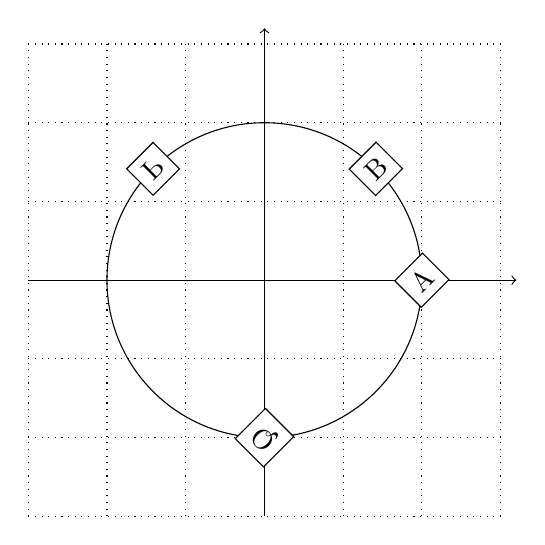
\begin{tikzpicture}[transform shape, every node/.style={draw, fill=white}]
  \draw[thin,dotted] (-3,-3) grid (3,3);
  \draw[->] (-3,0) -- (3.2,0);
  \draw[->] (0,-3) -- (0,3.2);
  \draw circle(2);
  \node[xshift=2cm, rotate=45] {A};
  \node[rotate=45, xshift=2cm] {B};
  \node[rotate=45, yshift=2cm, yscale=-1] {P};
  \node[yscale=-1, yshift=2cm, rotate=45] {Q};
\end{tikzpicture}
\end{document}
